\section{A latent variable model for temporal data}

%%%%%%%%%%%%%%%%%%%%%%%%%%%%%%%%%%%%%%%%%%%%%%%%%%%%%%%%%%%%%%%

\begin{frame}{Let's talk about the weather}

\svspace{-5mm}

\begin{center}
	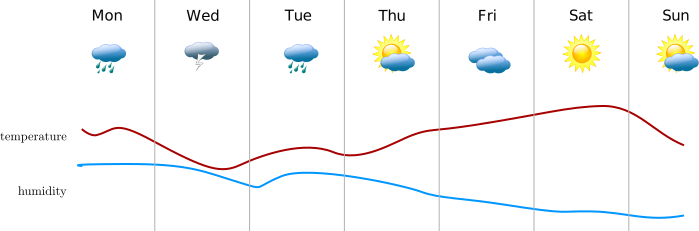
\includegraphics[width=0.7\textwidth]{img/weather}
\end{center}

\begin{center}
\slidesonly{
\only<2>{
	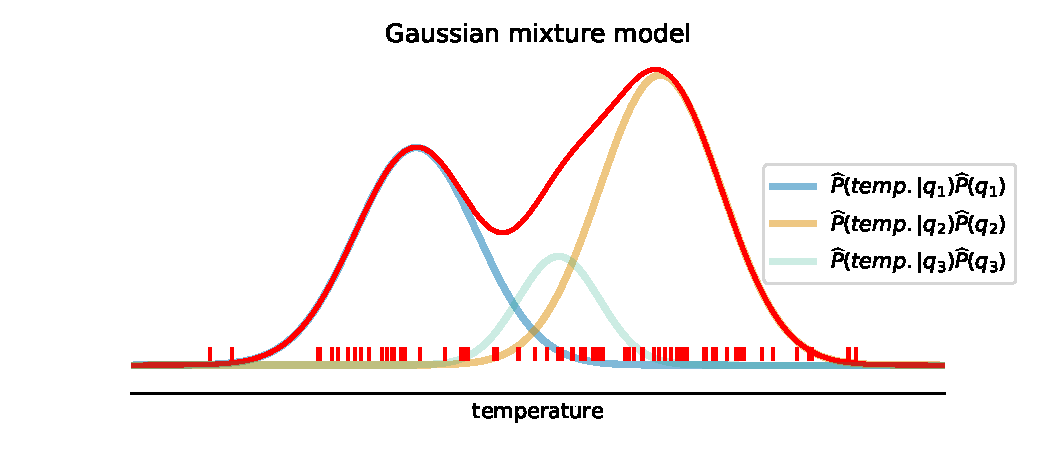
\includegraphics[width=0.6\textwidth]{img/latentexample_gmm_weather}
	}
}
\only<3>{
	\includegraphics<3>[width=0.6\textwidth]{img/latentexample_gmm_weather_icons}
}
	\notesonly{\captionof{figure}
	{A density estimation from a latent variable model}
	}\slidesonly{\captionof*{figure}
	{A density estimation from a latent variable model}
	}
\end{center}

\end{frame}

\begin{frame}{It's not all about amplitudes}

\begin{center}
	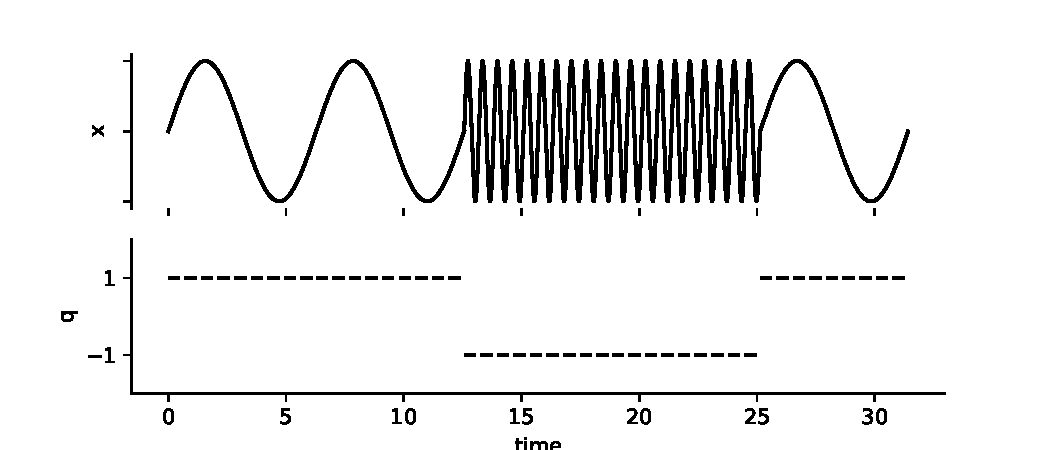
\includegraphics[width=0.9\textwidth]{img/sin}
\end{center}


\end{frame}

\begin{frame}

\begin{itemize}
\only<1->{
\item We have a sequence of observed events: $\vec x^{(t)} \in \R^N$
\item successive events $\vec x^{(t)}, \vec x^{(t-1)}$ \underline{cannot} be treated as independent
}
\slidesonly{
\svspace{10mm}
\only<2>{
\begin{minipage}{0.45\textwidth}
	\captionof*{figure}{at t=1}
	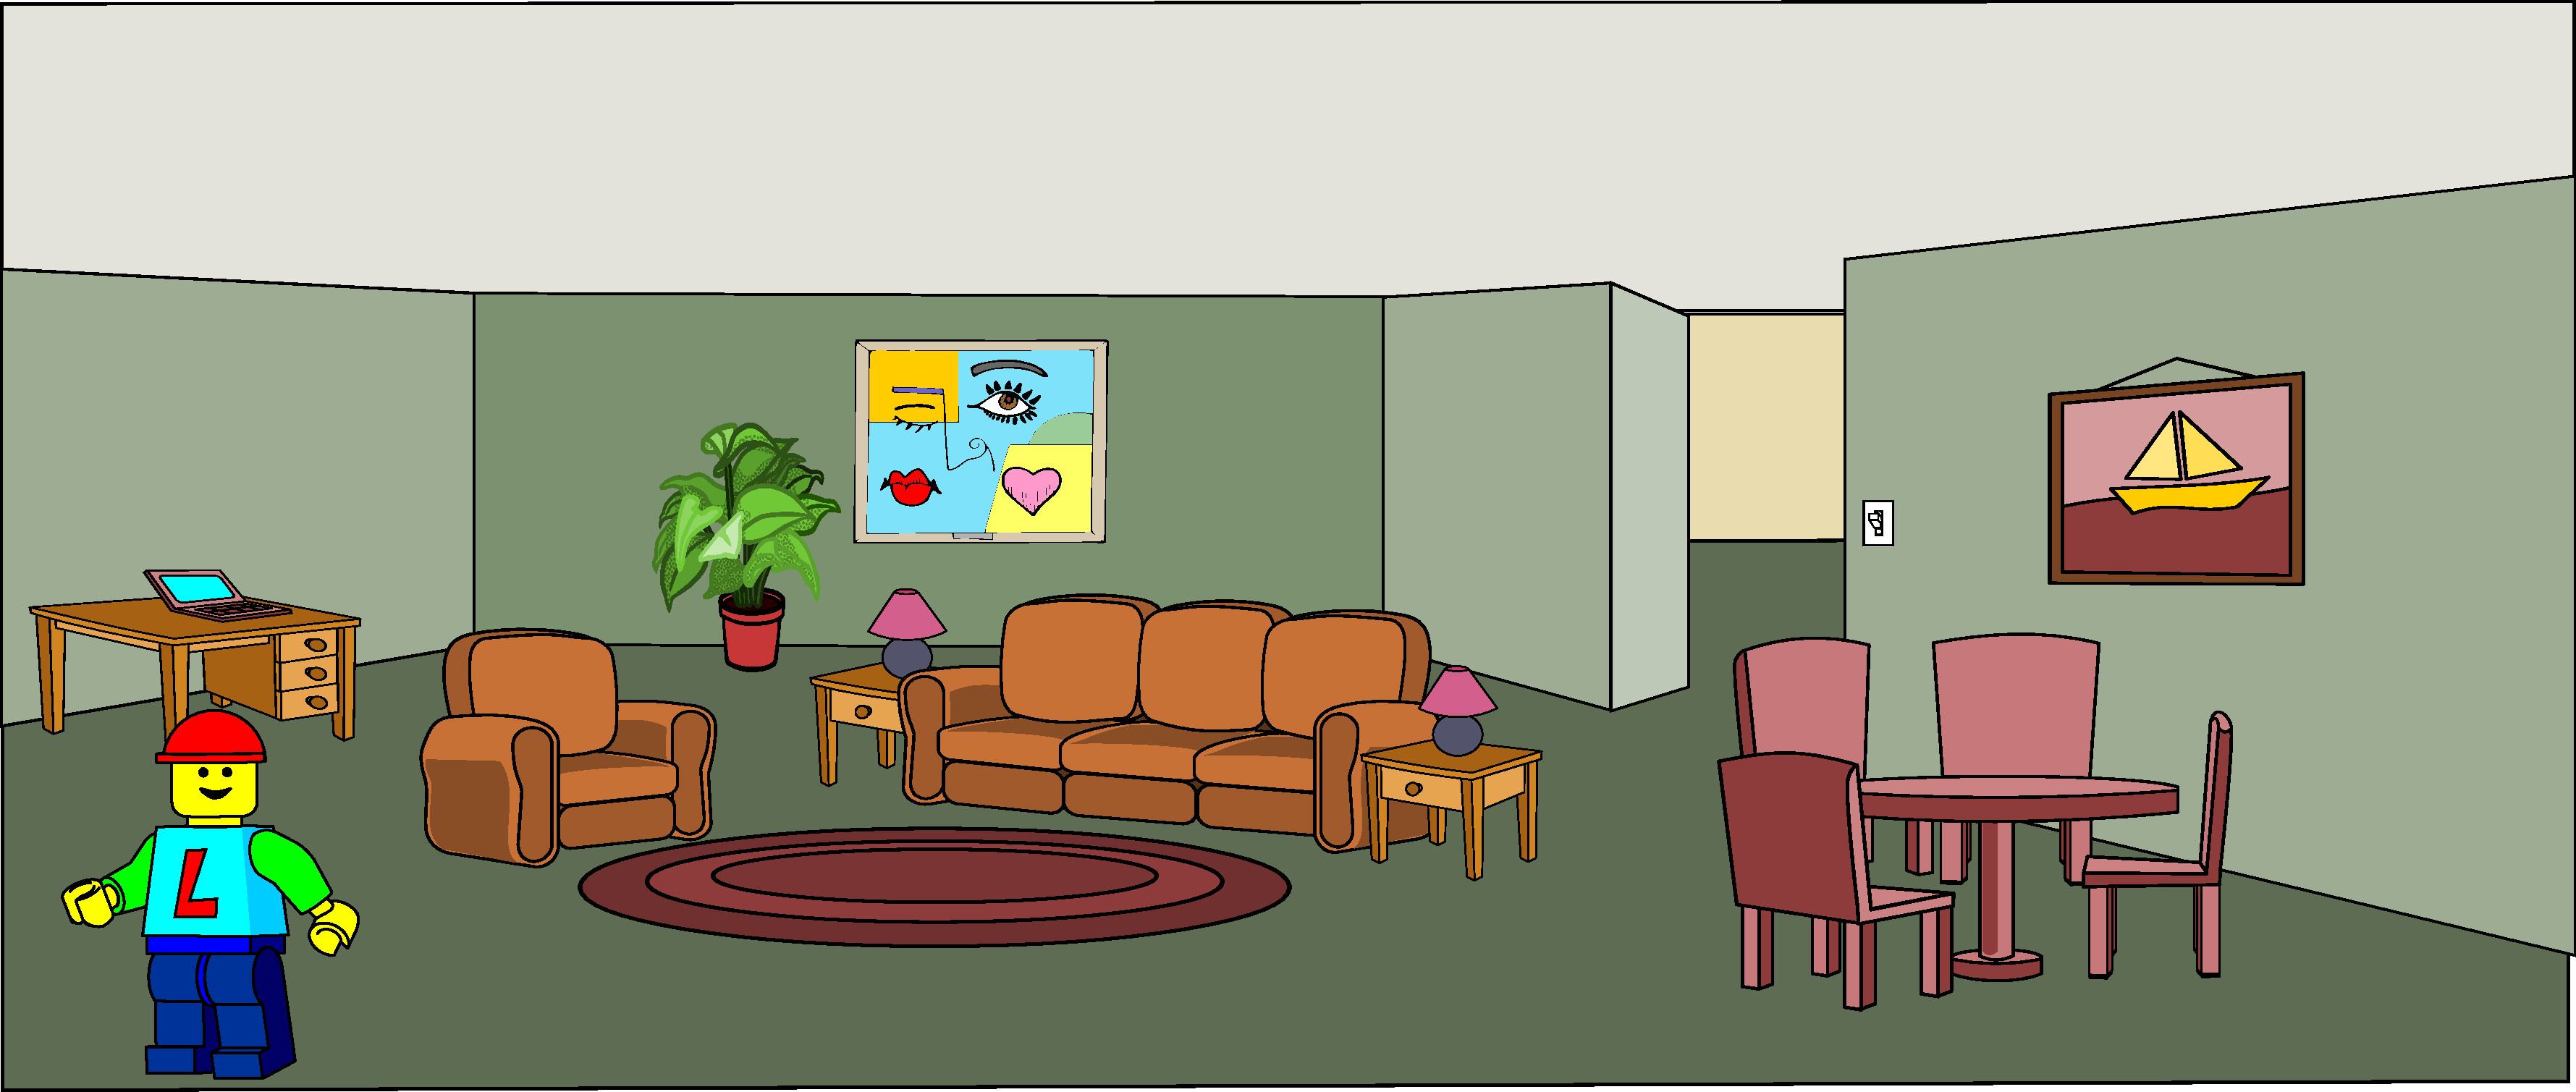
\includegraphics[width=0.99\textwidth]{img/Living-Room-Scene_001_figure_1}
\end{minipage}
\begin{minipage}{0.45\textwidth}
	\captionof*{figure}{at t=2}
	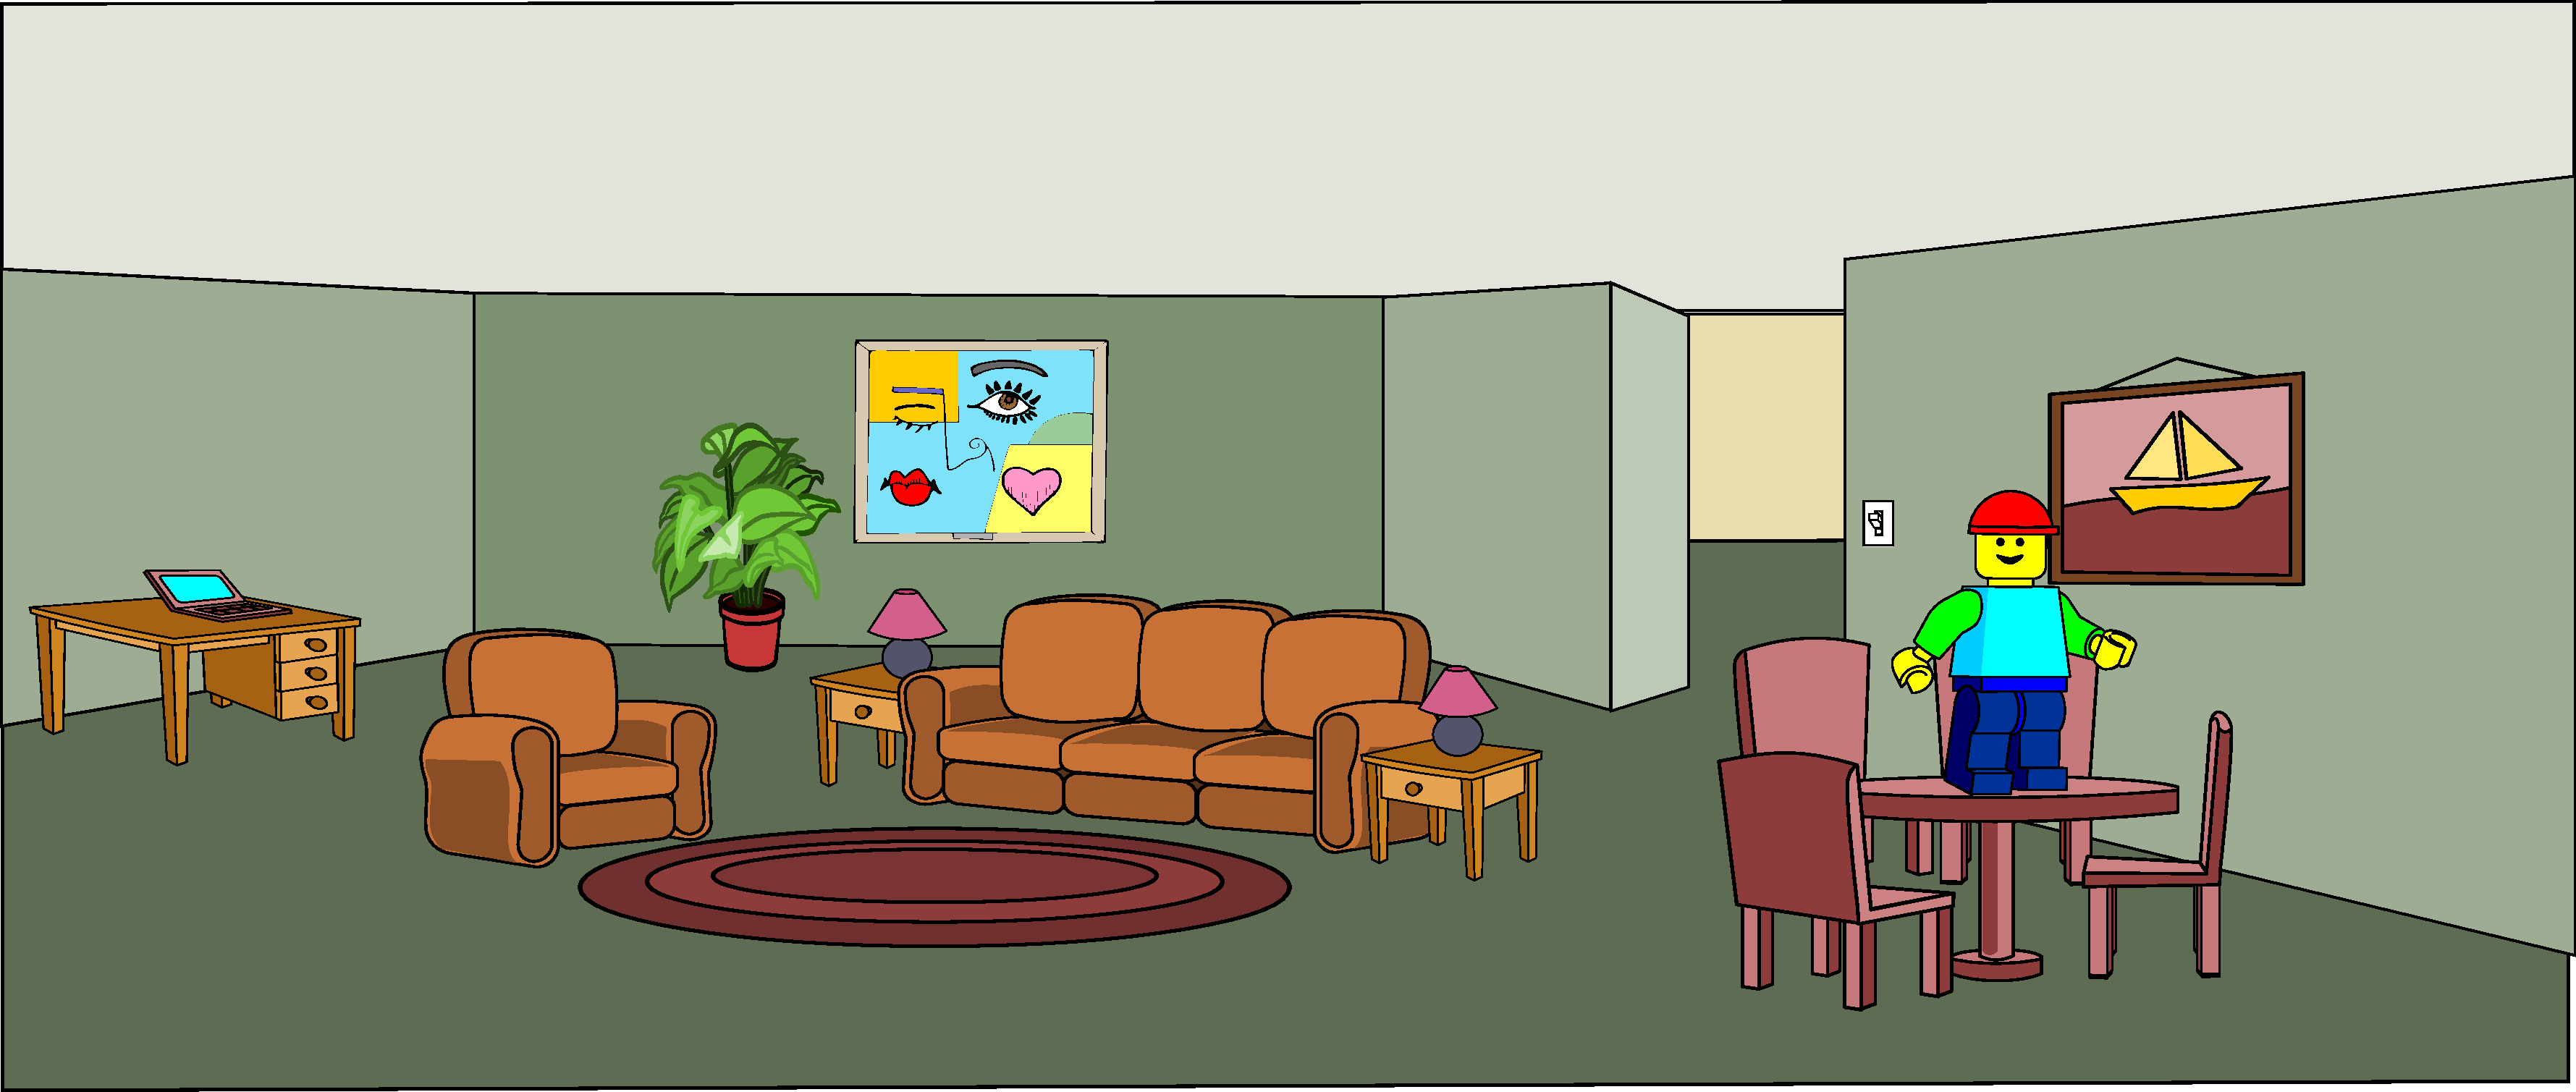
\includegraphics[width=0.99\textwidth]{img/Living-Room-Scene_001_figure_2}
\end{minipage}\\

\begin{minipage}{0.45\textwidth}
	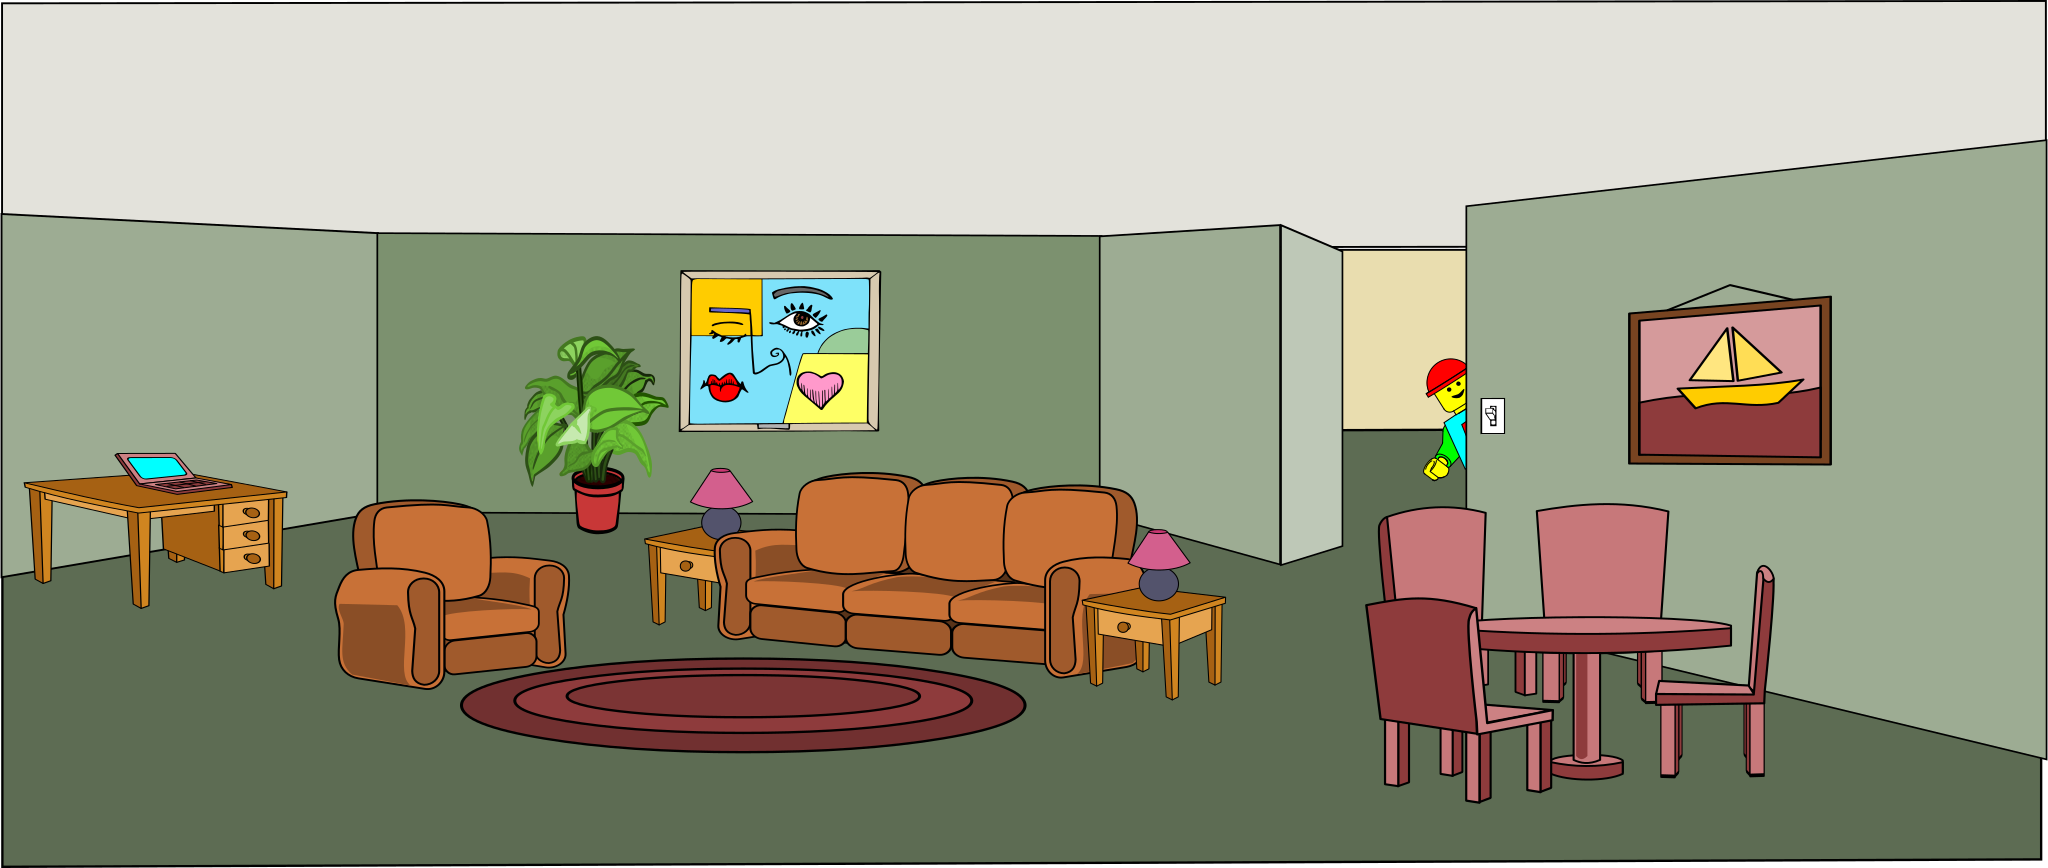
\includegraphics[width=0.99\textwidth]{img/Living-Room-Scene_001_figure_3}
	\captionof*{figure}{at t=3}
\end{minipage}
\begin{minipage}{0.45\textwidth}
	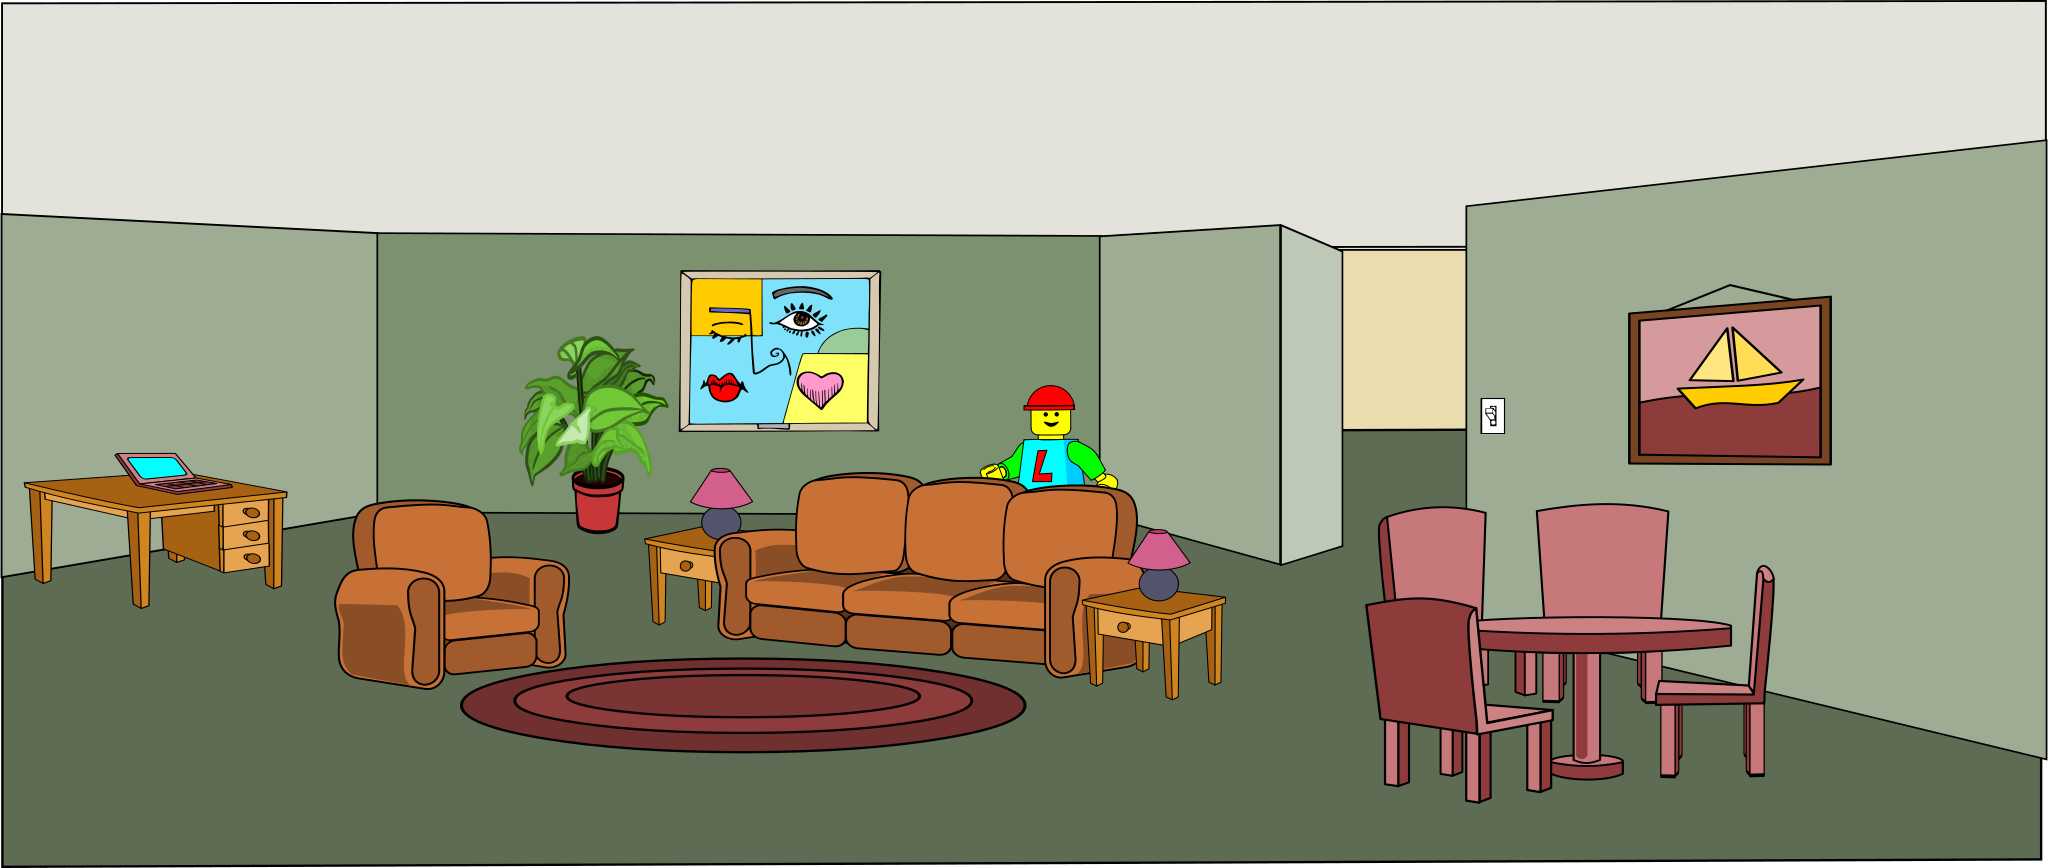
\includegraphics[width=0.99\textwidth]{img/Living-Room-Scene_001_figure_4}
	\captionof*{figure}{at t=4}
\end{minipage}
	}
}
\only<3->{
\item Assumption:\\
What we observe at every time step in the sequence $\{ \vec x^{(t)}\}_{t=1}^{T}$ is a result of the ``system'' being in a specific \emph{hidden state} at every time step $t$:\\
e.g. 1-out-of-$M$ coding for $M$ different states:
\begin{itemize} 
\item $\vec{m}^{(t)} = \big( m_1^{(t)}, \dots, m_M^{(t)} \big)^\top \in \left\{ 0, 1 \right\}^M$ \\
		\begin{align}
		m_q^{(t)} &= 
		\begin{cases}
		1, & \text{if system is in state } q \text{ at time}~t\\
		0, & \text{otherwise}
		\end{cases}
		%\hspace{0.5cm}
		\;\text{with} \;
		 \sum_{q=1}^{M} m_q^{(t)} = 1 
		\end{align}
\end{itemize}
\item Our observed sequence is a result of this \emph{hidden state} sequence
}
\end{itemize}

\end{frame}

\begin{frame}{Only}
\frametitle{Possibilities}

We may want to do:
\begin{itemize}
\item<only@1> Describe the sequence of hidden states:
$\{ \vec m^{(1)}, \ldots, \vec m^{(t)}, \ldots, \vec m^{(T)}\} = \{ \vec m^{(t)}\}_{t=1}^{T} \stackrel{\substack{\text{for}\\ \text{brevity}}}{=} \{ \vec m^{(t)}\}$
after observing the the sequence $\{\vec x^{(t)}\}$\\

\svspace{5mm}

\begin{center}
	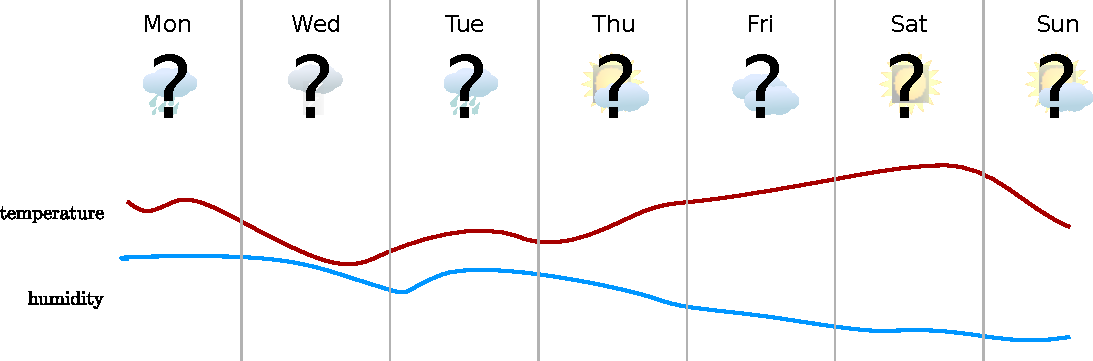
\includegraphics[width=0.7\textwidth]{img/weather_est_states}
	\notesonly{\captionof{figure}{Predict the sequence of hidden states}}
\end{center}

Example: hear sounds $\rightarrow$ what words were said? (transcribing speech)
\item<only@2> Generate a sequence of observations given a sequence of hidden variables $\{\vec m^{(t)}\}$
\\

\svspace{5mm}

\begin{center}
	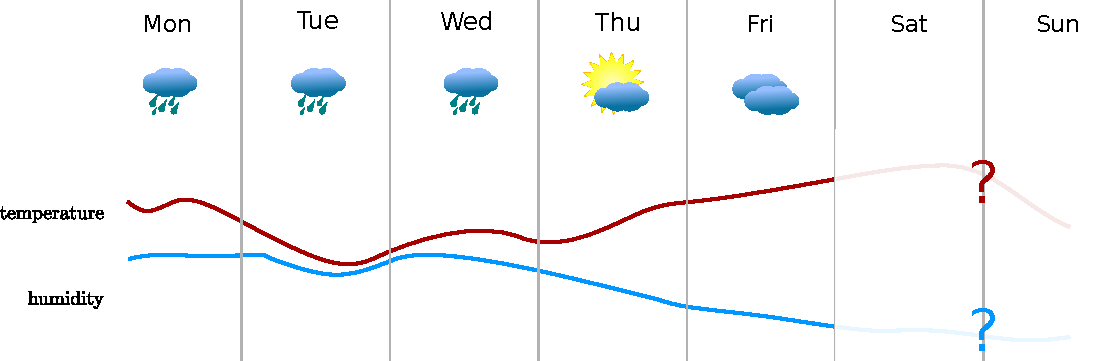
\includegraphics[width=0.7\textwidth]{img/weather_est_obs}
	\notesonly{\captionof{figure}{Predict the next sequence of observations}}
\end{center}

Example: type in words $\rightarrow$ hear speech (speech synthesis)
\item<only@3> Given a sequence $\{\vec x^{(t)}\}$ or $\{\vec m^{(t)}\}$ or both,\\
predict the next $\vec x$ and/or $\vec m$

\svspace{5mm}

\begin{center}
	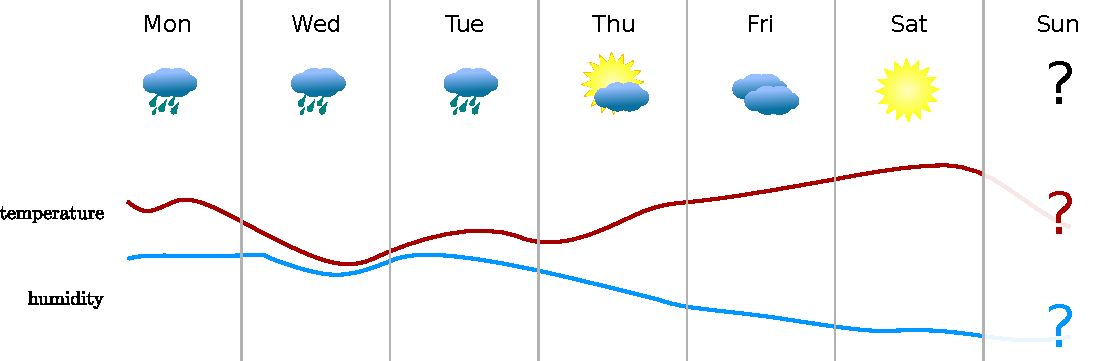
\includegraphics[width=0.7\textwidth]{img/weather_est_next}
	\notesonly{\captionof{figure}{Predict the next state and/or observation}}
\end{center}

\end{itemize}

\notesonly{
We can achieve all the above using Hidden Markov Models (HMM)
}

\end{frame}
